\documentclass[12pt]{standalone}

\usepackage{amsmath}

\usepackage{tikz-feynman}
\tikzfeynmanset{compat=1.1.0}

\newcommand{\A}{$a, \mu$}
\newcommand{\B}{$b, \nu$}
\newcommand{\C}{$c, \rho$}
\newcommand{\D}{$d, \sigma$}

\newcommand{\rhs}{
    $
    \begin{aligned}
        -i &g_s^2 [f^{abe} f^{cde} (g^{\mu\rho} g^{\nu\sigma} - g^{\mu\sigma} g^{\nu\rho}) \\
                &+ f^{ace} f^{bde} (g^{\mu\nu} g^{\rho\sigma} - g^{\mu\sigma} g^{\nu\rho}) \\
                &+ f^{ade} f^{bce} (g^{\mu\nu} g^{\rho\sigma} - g^{\mu\rho} g^{\nu\sigma})]
    \end{aligned}
    $
}

\begin{document}

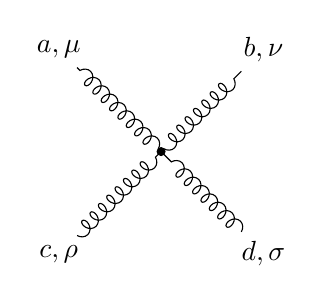
\begin{tikzpicture}[baseline=-\the\dimexpr\fontdimen22\textfont2\relax]
    \begin{feynman}[inline=(m)]
        \vertex[dot] (m) at ( 0, 0) {};
        \vertex (a) at (-1.3,-1.3) {\C};
        \vertex (b) at ( 1.3,-1.3) {\D};
        \vertex (c) at (-1.3, 1.3) {\A};
        \vertex (d) at ( 1.3, 1.3) {\B};
        \diagram* {
            (a) -- [gluon] (m) -- [gluon] (c),
            (b) -- [gluon] (m) -- [gluon] (d),
        };
    \end{feynman}
\end{tikzpicture}

% $$
%   \begin{tikzpicture}[baseline=-\the\dimexpr\fontdimen22\textfont2\relax]
%       \begin{feynman}[inline=(m)]
%             \vertex[dot] (m) at ( 0, 0) {};
%             \vertex (a) at (-1.3,-1.3) {\C};
%             \vertex (b) at ( 1.3,-1.3) {\D};
%             \vertex (c) at (-1.3, 1.3) {\A};
%             \vertex (d) at ( 1.3, 1.3) {\B};
%             \diagram* {
%                   (a) -- [gluon] (m) -- [gluon] (c),
%                   (b) -- [gluon] (m) -- [gluon] (d),
%             };
%       \end{feynman}
%   \end{tikzpicture}
%   $=$ \rhs
% $$

\end{document}